\section {The arduino components}
\begin {frame} {Outline}
    \tableofcontents [current]
\end {frame}

\begin {frame} {The arduino components}
	Arduino kits can include :
	\begin{itemize}
		\item a breadboard
		\pause
		\item wooden base, pushbuttons, diodes, leds, wires
		\pause
		\item several resistors (and resistance values), capacitors
		\pause
		\item photo and temperature sensors
		\pause
		\item motors, transistors, …
	\end{itemize}
\end {frame}

\begin{frame}{The arduino components}
	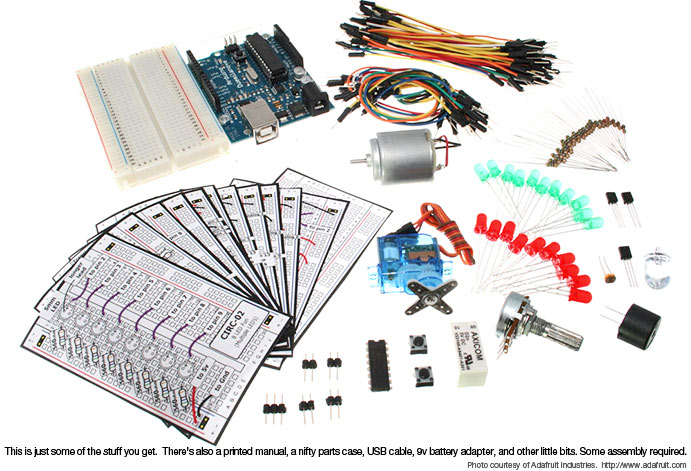
\includegraphics [width=1.0\textwidth,keepaspectratio] {img/components}
\end{frame}

\begin{frame}{The shields}
	\begin{itemize}
		\item Ethernet / WiFi / GPS / Wave
		\item Sensors
		\item NFC / RFID / SD card
		\item LCD
		\item …
		% There is no real limit, you just do whatever you can do with the power supplied by arduino
	\end{itemize}
\end{frame}

\begin{frame}{Stacked shields}
	\begin{center}
		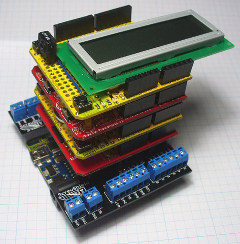
\includegraphics [width=0.5\textwidth,keepaspectratio] {img/stacked-shields}
	\end{center}
\end{frame}

%%%% TODO : add images
